\documentclass[12pt]{article}

%%%%%%%%%%%%%%%%%%%%%%%%%%%%%%%%%%%%%%%%%%%%%%%%%%%%%%%%%%%%%%%%%%%%%%%%%%%%%%%%%%%%%%%%%%%%%%%%%%%%
% Math
\usepackage{fancyhdr} 
\usepackage{amsfonts}
\usepackage{amsmath}
\usepackage{amssymb}
\usepackage{amsthm}
%\usepackage{dsfont}

%%%%%%%%%%%%%%%%%%%%%%%%%%%%%%%%%%%%%%%%%%%%%%%%%%%%%%%%%%%%%%%%%%%%%%%%%%%%%%%%%%%%%%%%%%%%%%%%%%%%
% Macros
\usepackage{calc}

%%%%%%%%%%%%%%%%%%%%%%%%%%%%%%%%%%%%%%%%%%%%%%%%%%%%%%%%%%%%%%%%%%%%%%%%%%%%%%%%%%%%%%%%%%%%%%%%%%%%
% Commands and Custom Variables	
\newcommand{\problem}[1]{\hspace{-4 ex} \large \textbf{Problem #1} }
%\let\oldemptyset\emptyset
%\let\emptyset\varnothing
\newcommand{\norm}[1]{\left\lVert#1\right\rVert}
\newcommand{\sint}{\text{s}\kern-5pt\int}
\newcommand{\powerset}{\mathcal{P}}
\renewenvironment{proof}{\hspace{-4 ex} \emph{Proof}:}{\qed}
\newcommand{\solution}{\textit{Solution}:\bigbreak}
\newcommand{\RR}{\mathbb{R}}
\newcommand{\NN}{\mathbb{N}}
\newcommand{\QQ}{\mathbb{Q}}
\newcommand{\ZZ}{\mathbb{Z}}
\newcommand{\CC}{\mathbb{C}}
\newcommand{\VV}{\mathbb{V}}
\newcommand{\FF}{\mathbb{F}}
\renewcommand{\Re}{\operatorname{Re}}
\renewcommand{\Im}{\operatorname{Im}}

\newcommand{\bigO}{\mathcal{O}}

\newcommand{\PP}{\mathcal{P}}
\newcommand{\LL}{\mathcal{L}}

\renewcommand{\vec}[1]{\boldsymbol{\mathbf{#1}}}

\newcommand{\editnote}[1]{\textcolor{red}{\textbf{\MakeUppercase{#1}}}}


%%%%%%%%%%%%%%%%%%%%%%%%%%%%%%%%%%%%%%%%%%%%%%%%%%%%%%%%%%%%%%%%%%%%%%%%%%%%%%%%%%%%%%%%%%%%%%%%%%%%
%page
\usepackage[margin=1in]{geometry}
\usepackage{setspace}
%\doublespacing
\allowdisplaybreaks
\pagestyle{fancy}
\fancyhf{}
\rhead{Shaw \space \thepage}
\setlength\parindent{0pt}
\usepackage{color}
\usepackage{enumerate}

%%%%%%%%%%%%%%%%%%%%%%%%%%%%%%%%%%%%%%%%%%%%%%%%%%%%%%%%%%%%%%%%%%%%%%%%%%%%%%%%%%%%%%%%%%%%%%%%%%%%
%Code
\usepackage{listings}
\usepackage{courier}
\lstset{
	language=Python,
	showstringspaces=false,
	formfeed=newpage,
	tabsize=4,
	commentstyle=\itshape,
	basicstyle=\ttfamily,
}

%%%%%%%%%%%%%%%%%%%%%%%%%%%%%%%%%%%%%%%%%%%%%%%%%%%%%%%%%%%%%%%%%%%%%%%%%%%%%%%%%%%%%%%%%%%%%%%%%%%%
%Images
\usepackage{graphicx}
\graphicspath{ {images/} }
\usepackage{float}

%tikz
\usepackage[utf8]{inputenc}
%\usepackage{pgfplots}
%\usepgfplotslibrary{groupplots}

%%%%%%%%%%%%%%%%%%%%%%%%%%%%%%%%%%%%%%%%%%%%%%%%%%%%%%%%%%%%%%%%%%%%%%%%%%%%%%%%%%%%%%%%%%%%%%%%%%%%
%Hyperlinks
%\usepackage{hyperref}
%\hypersetup{
%	colorlinks=true,
%	linkcolor=blue,
%	filecolor=magenta,      
%	urlcolor=cyan,
%}

\begin{document}
	\thispagestyle{empty}
	
	\begin{flushright}
		Sage Shaw \\
		m503 - Fall 2018 \\
		\today
	\end{flushright}
	
\begin{center}{\large \textbf{Possible Exam 2}}\end{center}
\bigbreak

\hspace{-.5 ex}\problem{1} Consider the space $\PP_2(\RR)$ and the function $\langle \cdot, \cdot \rangle : \PP_2(\RR) \times \PP_2(\RR) \to \RR$ given by
\begin{align}
\langle p, q \rangle = \int_{-1}^{1} p(x) q(x) x^2 dx\label{inner1}
\end{align}
For $p,q,r \in \PP_2(\RR)$ and $\lambda \in \RR$ prove the following:
\begin{enumerate}[(a)]
	\item \textbf{additivity in the first slot}: $\langle p+q, r \rangle = \langle p,r\rangle + \langle q,r\rangle$ \\
	\textbf{homogeneity in the first slot}: $\langle \lambda p, q \rangle = \lambda \langle p,q\rangle$\\ \textbf{conjugate symmetry}: $\langle p, q \rangle = \overline{\langle q,p\rangle}$ \bigbreak
	
	\item \textbf{positive definite}: $\langle p, p \rangle \geq 0$ and $\langle p, p \rangle=0 \iff p=0$. \\(Note that $(1, x, x^2)$ form a basis.) \textit{This might be Analysis heavy. Perhaps it should be extra credit.}\\
	\item Is $\langle \cdot, \cdot \rangle$ an inner product on $\PP_2(\RR)$?
\end{enumerate}

\pagebreak
%%%%%%%%%%%%%%%%%%%%%%%%%%%%%%%%%%%%%%%%%%%%%%%%%%%%%%%%%%%%%%%%%%%%%%%%%%%%%%%%%%%%%%%%%%%
\problem{2} Consider the space $\PP_2(\RR)$ and the function $\langle \cdot, \cdot \rangle : \PP_2(\RR) \times \PP_2(\RR) \to \RR$ given by
\begin{align}
\langle p, q \rangle = \int_{-1}^{1} p(x) q(x) x dx\label{inner2}
\end{align}
Calculate the following:
\begin{enumerate}
	\item $\langle 1, 1 \rangle$
	\item $\langle x, x \rangle$
	\item $\langle x^2, x^2 \rangle$
\end{enumerate}
Is $\langle \cdot, \cdot \rangle$ an inner product?

\pagebreak
%%%%%%%%%%%%%%%%%%%%%%%%%%%%%%%%%%%%%%%%%%%%%%%%%%%%%%%%%%%%%%%%%%%%%%%%%%%%%%%%%%%%%%%%%%%
\problem{3} Find an orthogonal basis for $\PP_2(\RR)$ with respect to the inner product given in (\ref{inner1}).


\pagebreak
%%%%%%%%%%%%%%%%%%%%%%%%%%%%%%%%%%%%%%%%%%%%%%%%%%%%%%%%%%%%%%%%%%%%%%%%%%%%%%%%%%%%%%%%%%%
\problem{4} Let $V, U$, and $W$ be vector spaces. Let $T \in \LL(U,V), S \in \LL(V,W)$. Draw a diagram that includes $T, S, T^*, S^*, S \circ T$, and $(S \circ T)^*$.

\pagebreak
%%%%%%%%%%%%%%%%%%%%%%%%%%%%%%%%%%%%%%%%%%%%%%%%%%%%%%%%%%%%%%%%%%%%%%%%%%%%%%%%%%%%%%%%%%%
\problem{5} Define $T: \RR^2 \to \RR^2$ as 
$$
T(\vec{x}) = \begin{bmatrix}0&-1\\1&0\end{bmatrix}\vec{x}
$$
and find $T^*$ with respect to the standard inner product on $\RR^2$:
$$
\left\langle \begin{bmatrix}x_1\\y_1\end{bmatrix}, \begin{bmatrix}x_2\\y_2\end{bmatrix} \right \rangle = x_1x_2 + y_1y_2.
$$
\ 
\bigbreak \ 
\bigbreak \ 
\bigbreak \ 
\bigbreak \ 

Find $T^*$ with respect to the following (weighted) inner product:
\begin{align}
\left\langle \begin{bmatrix}x_1\\y_1\end{bmatrix}, \begin{bmatrix}x_2\\y_2\end{bmatrix} \right \rangle =
\begin{bmatrix}x_2&y_2\end{bmatrix}
\begin{bmatrix}1&1\\0&1\end{bmatrix}
\begin{bmatrix}x_1 \\ y_1 \end{bmatrix}
= x_{1} x_{2} + y_{2} \left(x_{1} + y_{1}\right) \label{inner5}
\end{align}

\pagebreak
%%%%%%%%%%%%%%%%%%%%%%%%%%%%%%%%%%%%%%%%%%%%%%%%%%%%%%%%%%%%%%%%%%%%%%%%%%%%%%%%%%%%%%%%%%%
\problem{6} Consider the vector space $V=\RR^2$ under the inner product given in (\ref{inner5}). Let $U\subseteq V$ be the line $y = x$. Find $U^\perp$ and sketch both $U$ and $U^\perp$.

\pagebreak
%%%%%%%%%%%%%%%%%%%%%%%%%%%%%%%%%%%%%%%%%%%%%%%%%%%%%%%%%%%%%%%%%%%%%%%%%%%%%%%%%%%%%%%%%%%
\problem{7} Suppose we wish to approximate the function $f(x) = \sin(x)$ over the interval $[-2\pi,2\pi]$ with a polynomial. We will consider 3 polynomials as good candidates: 
\begin{enumerate}
	\item $T_9(x)$ - the 9th degree Taylor Series.
	\begin{figure}[H]
		%\caption{Equispaced points}
		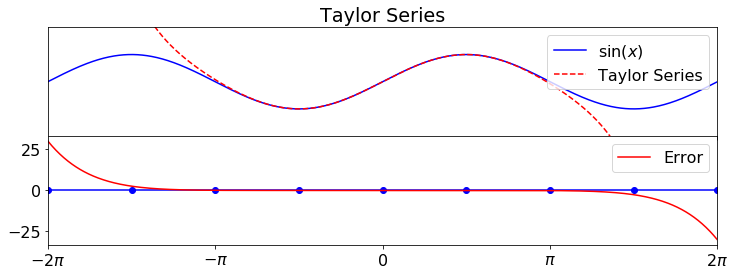
\includegraphics[width=1\textwidth]{taylor}
		\centering
	\end{figure}
	\item $P_9(x)$ - the polynomial that interpolates at 9 equally spaced points.
	\begin{figure}[H]
		%\caption{Equispaced points}
		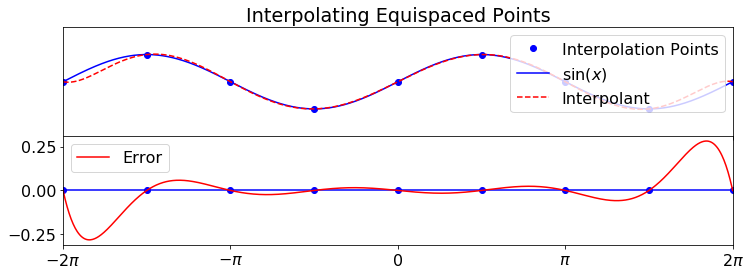
\includegraphics[width=1\textwidth]{equispaced}
		\centering
	\end{figure}
	\item $Q_9(x)$ - the polynomial that interpolates at 9 Chebyshev points.
	\begin{figure}[H]
		%\caption{Equispaced points}
		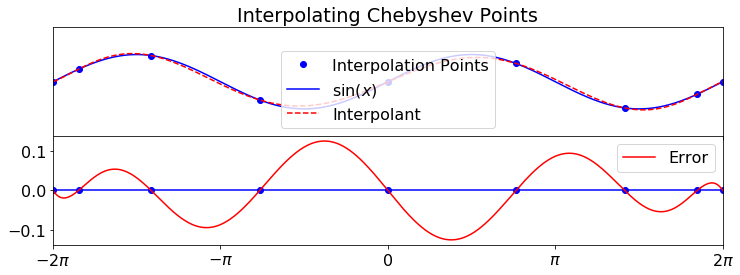
\includegraphics[width=1\textwidth]{chebyshev}
		\centering
	\end{figure}
\end{enumerate}

If we wish to compare these approximations, we must define a norm on continuous real-valued functions in order to say which is a ``closer" approximation. Specifically, if we have two polynomials $p(x), q(x)$, and a norm $\norm{\cdot}$,  we say that $p$ is a better approximation than $q$ under the given norm, if $\norm{p - f} < \norm{q - f}$. We consider the following inner products on continuous functions, and their induced norms:
\begin{align*}
	\langle f, g \rangle_2 & = \int_{-2\pi}^{2\pi} f(x)g(x) dx & \norm{f}_2 &= \sqrt{\int_{-2\pi}^{2\pi} \vert f(x) \vert^2 dx} & \tag{Euclidian Norm} \\
	 &  \text{(N/A)} & \norm{f}_\infty &= \max_{x \in [-2\pi, 2\pi]}\{f(x)\} & \tag{Max Norm} \\
	\langle f, g \rangle_* & = \int_{\pi}^{\pi} f(x)g(x) dx & \norm{f}_* &= \sqrt{\int_{-\frac{3}{2}\pi}^{\frac{3}{2}\pi} \vert f(x) \vert^2 dx} & \tag{Interior Norm} \\
\end{align*}
The $\norm{\cdot}_2$ norm can be though of as a least squares goodness of fit, giving larger error more weight than smaller error over over the same length. The $\norm{\cdot}_\infty$ can be thought of as measuring the maximum error. Note that there is no inner-product that will induce this norm, but it is a valid norm on continuous functions over closed intervals. Lastly $\norm{\cdot}_*$ is not concerned with error near the boundary. The approximating polynomials and their errors are shown in the same plot below for ease of comparison.

\begin{figure}[H]
	%\caption{Equispaced points}
	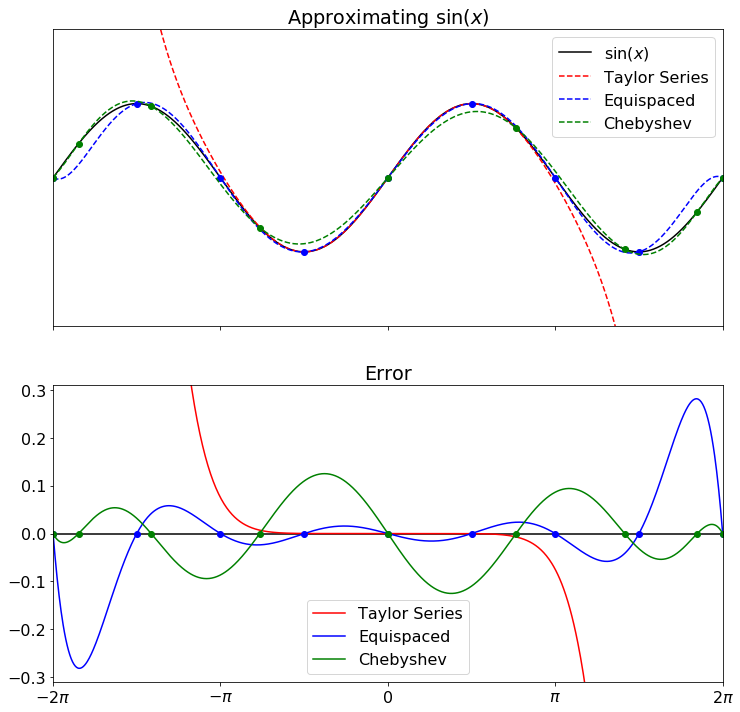
\includegraphics[width=1\textwidth]{approx}
	\centering
\end{figure}

\pagebreak
Which of the following seems true? Justify your answers.
\begin{enumerate}[(a)]
	\item $\norm{T_9-f}_2 < \norm{P_9-f}_2 < \norm{Q_9-f}_2$ (Equispaced interpolation is better.)
	\item $\norm{T_9-f}_2 < \norm{Q_9-f}_2 < \norm{P_9-f}_2$ (Chebyshev interpolation is better.)\\\\\\\\
	
	\item $\norm{T_9-f}_\infty < \norm{P_9-f}_\infty < \norm{Q_9-f}_\infty$ 
	\item $\norm{T_9-f}_\infty < \norm{Q_9-f}_\infty < \norm{P_9-f}_\infty$ \\\\\\\\
	
	\item $\norm{T_9-f}_* < \norm{P_9-f}_* < \norm{Q_9-f}_*$ 
	\item $\norm{T_9-f}_* < \norm{Q_9-f}_* < \norm{P_9-f}_*$ \\\\\\\\
\end{enumerate}




\end{document}
